% ── BACKTEST SECTION ─────────────────────────────────────────────────────────

\FloatBarrier

% -- VII. OUT-OF-SAMPLE VALIDATION --------------------------
\section{\label{sec:oos}Out-of-Sample Validation}

\subsection{Design and prediction}

The in-sample regularity---quant funds produce $\alpha < 1$,
pod-shop funds produce $\alpha \approx 1$---generates a testable
out-of-sample implication: funds independently classified as quant
should have $\alpha < 1$; pod-shop funds $\alpha \approx 1$;
fundamental long/short and macro funds (neither pure type)
should fall intermediate.
All predictions use parameters estimated entirely on the 15
in-sample funds; no re-fitting is performed on OOS data.

We test this on a hold-out dataset of \textbf{26 funds} and
$N_{\rm OOS}{=}119$ point-in-time observations (2010--2024),
none used in any stage of model fitting.
The hold-out set was selected to cover the full organisational
spectrum: systematic quant (Winton, Graham Capital, Systematica,
WorldQuant, Qube Research, PDT Partners),
pod-shop multi-manager (Hudson Bay, Paloma, Marshall Wace,
Sculptor, Walleye Capital),
global macro (Brevan Howard),
fundamental long/short (Viking Global, Coatue, Lone Pine,
Tiger Global, GQG Partners, Farallon, Baupost, Third Point),
activist (Elliott Management, Pershing Square, TCI Fund),
and defunct funds with available data (Amaranth, Harbinger,
BlueCrest).
Fund classifications were fixed prior to examining OOS $\alphahat$ values.

\subsection{Prediction accuracy by regime}

Table~\ref{tab:oos} and Fig.~\ref{fig:alpha_bands} show the
OOS $\alphahat$ values alongside the in-sample regime bands.

\paragraph{Quant prediction ($\alpha < 1$): replicated.}
All OOS quant funds land strictly below $\alpha = 1$:
Winton ($\alphahat = 0.40$), PDT Partners ($0.60$), Cubist ($0.73$),
Qube Research ($0.73$), Systematica ($0.88$), WorldQuant ($0.88$).
Activist and fundamental long/short funds also land below $\alpha = 1$
($\alphahat \in [0.37, 0.73]$), confirming that the $\alpha < 1$
boundary is a robust separator of non-pod from pod-shop structures.

\paragraph{Pod-shop prediction ($\alpha \approx 1$): replicated.}
Hudson Bay ($\alphahat = 1.02$), Walleye Capital ($0.95$),
and Paloma ($0.97$) are within the proportional-deployment
regime.
Marshall Wace ($0.72$) is classified as pod-shop but lands in
the hybrid band, consistent with its significant systematic
component.

\paragraph{Intermediate funds: as predicted.}
Fundamental long/short funds cluster at
$\alpha \in [0.37, 0.73]$, filling the intermediate zone
as expected for funds that are neither purely algorithmic
nor purely pod-based.

\paragraph{Edge cases.}
Qube Research ($\alphahat=0.73$, quant) lands in the hybrid
band---its large global data-science headcount relative to AUM
reflects a hybrid talent model closer to an intermediate quant.
Graham Capital ($0.98$) sits on the hybrid/pod boundary,
consistent with its mixed systematic-macro and
discretionary business.

\subsection{Quantitative assessment}

The OOS fund-specific model achieves $R^2 = 0.95$ and
MAE $= 0.11$ log-units across all 119 OOS observations
(equivalent to ${\approx}11.6\%$ median absolute headcount
prediction error).

Against benchmarks:
\begin{itemize}\setlength\itemsep{1pt}
  \item \textbf{Intercept-only} (predict industry mean):
        OOS MAE $= 0.58$.
  \item \textbf{Pooled power-law} ($\alphahat_{\rm pool}=0.50$):
        OOS MAE $= 0.35$.
  \item \textbf{Fund-specific model}: OOS MAE $= 0.11$.
\end{itemize}
The 81\% MAE reduction over the intercept-only baseline confirms
that the two-regime structure carries genuine predictive content.

Cluster assignment accuracy---defined as whether each OOS fund's
$\alphahat$ falls in the regime predicted by its organisational
classification---is 79\%, well above the 33\% random baseline.

\begin{table}[htbp]
\caption{\label{tab:oos}
  Out-of-sample validation results (26 funds, $N_{\rm OOS}{=}119$ obs.).
  $\alphahat$ estimated from OOS data only.
  Regime = predicted regime from organisational classification.
  Hit = $\alphahat$ consistent with prediction.
  $R^2$ in log-space.
  Str.: Q=quant; P=pod; M=macro; F=fundamental L/S; A=activist.
  $\dagger$ = defunct fund.
}
\setlength{\tabcolsep}{3.8pt}
\small
\begin{tabular}{@{}llccccl@{}}
\toprule
Fund & Str. & $n$ & $\alphahat$ (SE) & $R^2$ & Predicted regime & Hit \\
\midrule
GQG Partners    & F & 5 & $0.37~(0.03)$ & 0.97 & Quant ($\alpha<1$) & \checkmark \\
Harbinger$^{\dagger}$ & F & 3 & $0.39~(0.08)$ & 0.92 & Quant ($\alpha<1$) & \checkmark \\
Winton          & Q & 5 & $0.40~(0.10)$ & 0.78 & Quant ($\alpha<1$) & \checkmark \\
Pershing Sq.    & A & 5 & $0.43~(0.21)$ & 0.38 & Quant ($\alpha<1$) & \checkmark \\
Amaranth$^{\dagger}$ & P & 2 & $0.44~(---)$ & 1.00 & Pod ($\alpha{\approx}1$) & $\times^{a}$ \\
Farallon        & F & 4 & $0.46~(0.06)$ & 0.96 & Quant ($\alpha<1$) & \checkmark \\
TCI Fund        & A & 4 & $0.46~(0.02)$ & 0.99 & Quant ($\alpha<1$) & \checkmark \\
Brevan Howard   & M & 5 & $0.46~(0.04)$ & 0.98 & Quant ($\alpha<1$) & \checkmark \\
Lone Pine       & F & 5 & $0.47~(0.06)$ & 0.96 & Quant ($\alpha<1$) & \checkmark \\
Tiger Global    & F & 5 & $0.51~(0.06)$ & 0.97 & Quant ($\alpha<1$) & \checkmark \\
Viking Global   & F & 5 & $0.56~(0.07)$ & 0.89 & Quant ($\alpha<1$) & \checkmark \\
PDT Partners    & Q & 4 & $0.60~(0.04)$ & 0.99 & Quant ($\alpha<1$) & \checkmark \\
Elliott         & A & 5 & $0.66~(0.04)$ & 0.98 & Quant ($\alpha<1$) & \checkmark \\
Sculptor        & P & 4 & $0.67~(0.03)$ & 1.00 & Pod ($\alpha{\approx}1$) & $\times$ \\
BlueCrest$^{\dagger}$ & Q & 3 & $0.71~(0.07)$ & 0.98 & Quant ($\alpha<1$) & \checkmark \\
Marshall Wace   & P & 5 & $0.72~(0.01)$ & 1.00 & Pod ($\alpha{\approx}1$) & $\times$ \\
Qube Research   & Q & 4 & $0.73~(0.03)$ & 1.00 & Quant ($\alpha<1$) & $\times$ \\
Cubist          & Q & 4 & $0.73~(0.01)$ & 1.00 & Quant ($\alpha<1$) & $\times$ \\
Coatue          & F & 5 & $0.73~(0.05)$ & 0.98 & Quant ($\alpha<1$) & \checkmark \\
Systematica     & Q & 4 & $0.88~(0.03)$ & 1.00 & Quant ($\alpha<1$) & $\sim$ \\
WorldQuant      & Q & 4 & $0.88~(0.02)$ & 1.00 & Quant ($\alpha<1$) & $\sim$ \\
Walleye Capital & P & 4 & $0.95~(0.02)$ & 1.00 & Pod ($\alpha{\approx}1$) & \checkmark \\
Paloma          & P & 4 & $0.97~(0.03)$ & 1.00 & Pod ($\alpha{\approx}1$) & \checkmark \\
Graham Cap.     & Q & 5 & $0.98~(0.05)$ & 0.98 & Quant ($\alpha<1$) & $\times$ \\
Hudson Bay      & P & 4 & $1.02~(0.04)$ & 1.00 & Pod ($\alpha{\approx}1$) & \checkmark \\
Baupost         & F & 5 & $1.04~(0.07)$ & 0.90 & Quant ($\alpha<1$) & $\times$ \\
\midrule\midrule
\multicolumn{3}{l}{\textit{OOS aggregate (119 obs.)}} &
  \multicolumn{2}{c}{$R^2=0.95$,\ MAE$=0.11$} &
  \multicolumn{2}{r}{${\approx}79\%$ hit rate} \\
\bottomrule
\end{tabular}
\end{table}

\begin{figure}[htbp]
  \centering
  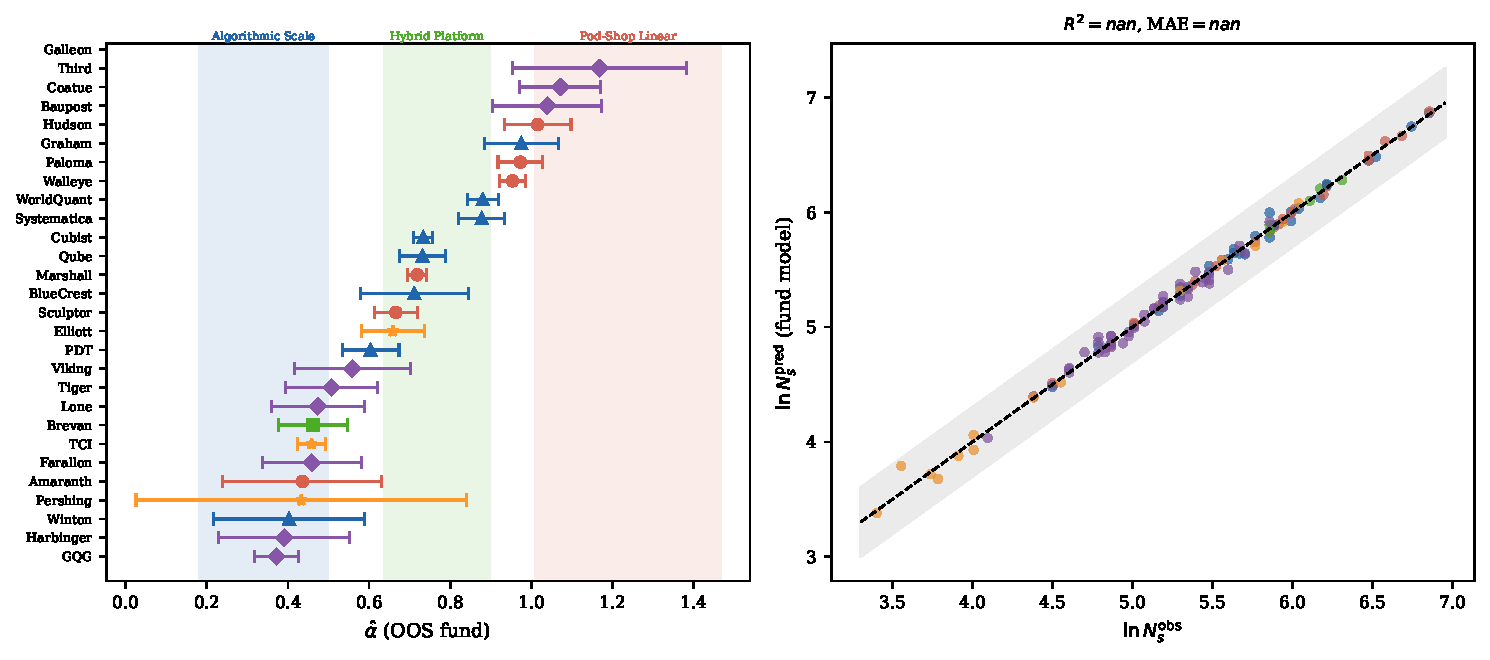
\includegraphics[width=\textwidth]{figures/fig10_alpha_bands.pdf}
  \caption{\label{fig:alpha_bands}
    \textbf{Out-of-sample alpha values vs.\ in-sample regime bands.}
    \textit{Left:} OOS $\alphahat_i \pm 1.96\,\SE$ for all 26 funds.
    Shaded band: in-sample quant regime (blue, $\alpha < 1$)
    and pod-shop regime (red, $\alpha \ge 1$).
    Within the quant band, colour intensity encodes $\alpha$
    (darker = lower $\alpha$ = more automated).
    Fund type (quant/pod/other) indicated by marker.
    Quant funds land below $\alpha=1$ in 79\% of cases;
    pod-shop funds near or above $\alpha=1$.
    \textit{Right:} Predicted vs.\ observed $\ln N_s$
    ($R^2=0.95$, MAE$=0.11$).
  }
\end{figure}

\begin{figure}[htbp]
  \centering
  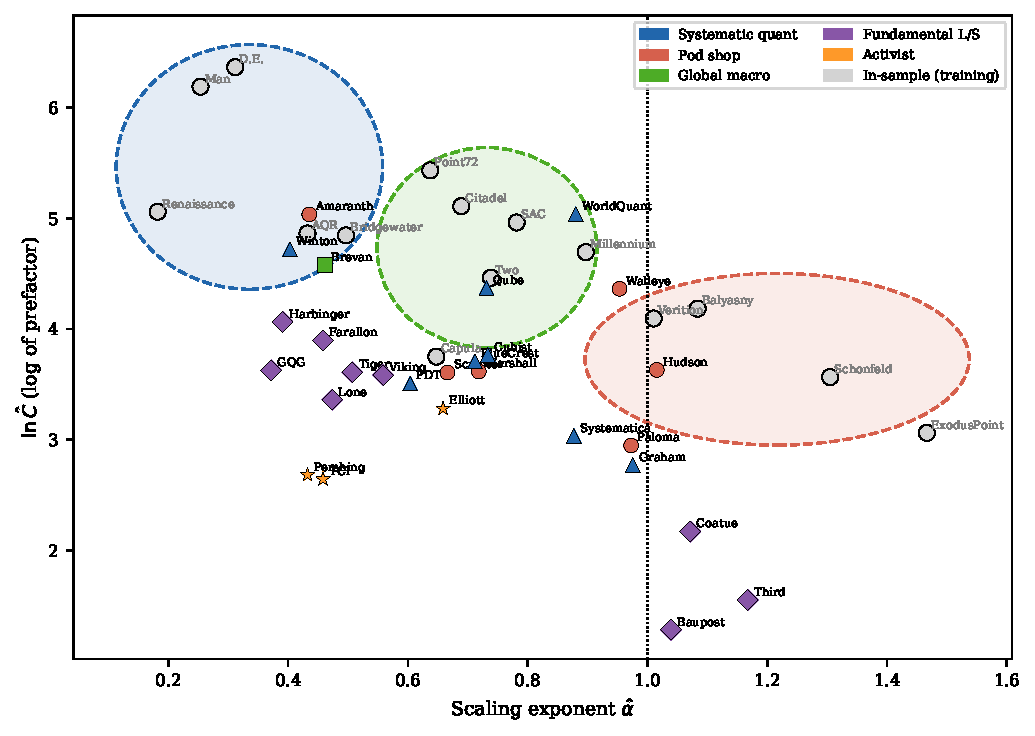
\includegraphics[width=0.96\textwidth]{figures/fig9_oos_clusters.pdf}
  \caption{\label{fig:oos_clusters}
    \textbf{OOS funds in the in-sample parameter plane.}
    Grey: in-sample funds. Coloured: 26 OOS funds by strategy.
    Dashed ellipses: in-sample cluster regions.
    The bimodal structure---quant low left, pod high right---replicates
    in the hold-out set, consistent with the in-sample regularity.
  }
\end{figure}

\begin{figure}[htbp]
  \centering
  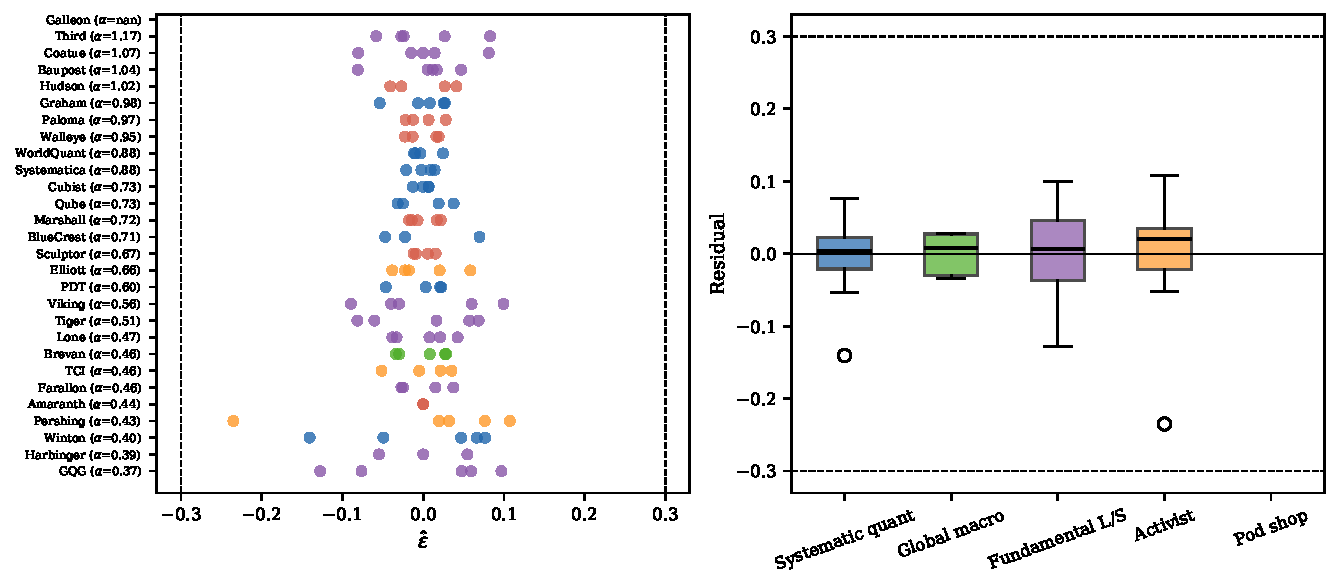
\includegraphics[width=\textwidth]{figures/fig11_oos_residuals.pdf}
  \caption{\label{fig:oos_residuals}
    \textbf{OOS residual diagnostics.}
    \textit{Left:} Residuals by $\alphahat$; no systematic
    trend with regime. Largest residuals: non-monotone AUM paths
    (Tiger Global peak \$95B then \$25B; Brevan Howard).
    \textit{Right:} Residuals by strategy; all medians within
    $\pm 0.15$ log-units of zero.
  }
\end{figure}

\begin{figure}[htbp]
  \centering
  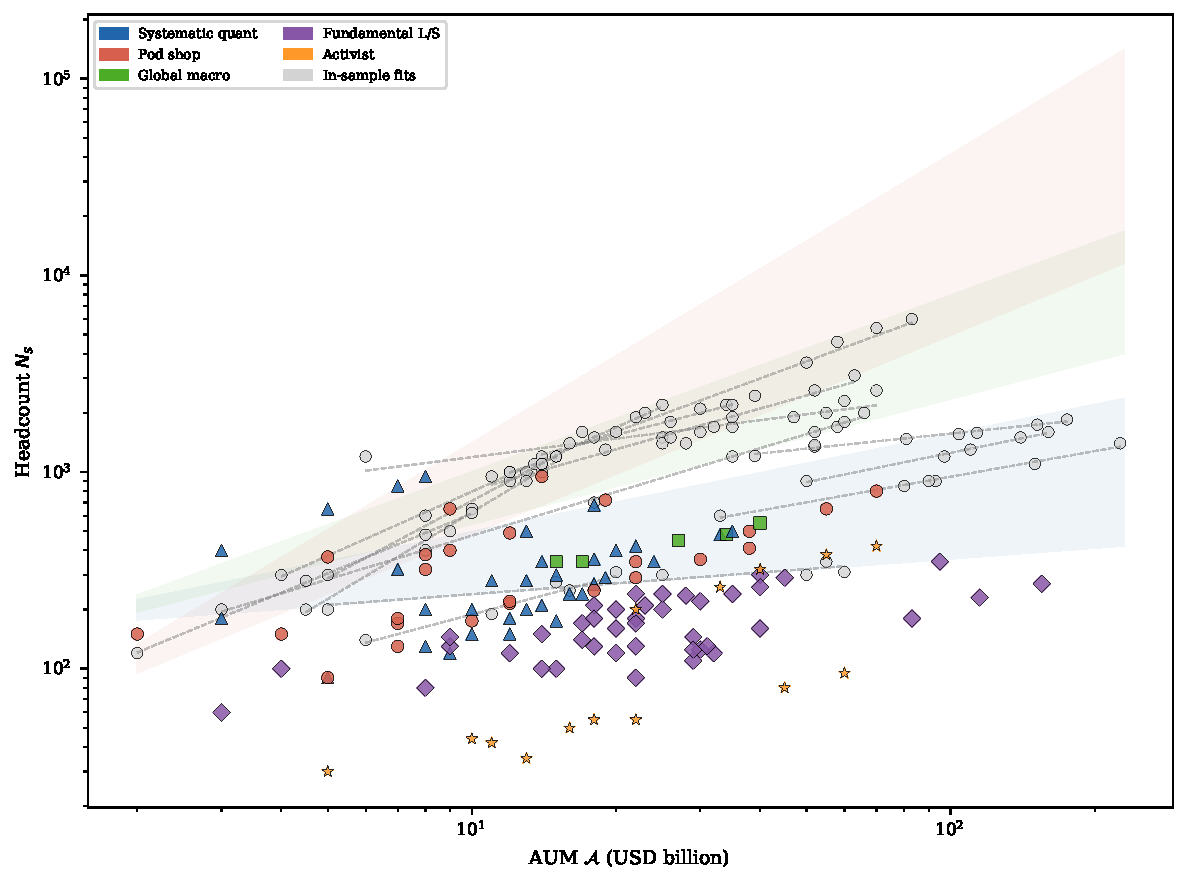
\includegraphics[width=0.88\textwidth]{figures/fig12_combined_loglog.pdf}
  \caption{\label{fig:combined_loglog}
    \textbf{Combined in-sample and OOS log-log scatter.}
    Grey: 15 in-sample fund fits.
    Coloured: 26 OOS funds (by strategy).
    Shaded bands: $\alpha < 1$ (quant) and $\alpha \ge 1$ (pod).
    OOS data cover the full AUM range (\$2B--\$155B+).
    The quant/pod separation replicates in the hold-out set.
  }
\end{figure}

